% !TEX root = ../../main.tex

\section{Processing a large adsorption dataset}

With the capability for fast processing
afforded by \texttt{pyGAPS}, we now turn to using it on an
available database of adsorption isotherms. The goal is to
test the speed and accuracy of the calculations, as well
as to obtain a description of the dataset. Further insights
may be obtained from benchmarking of different KPIs, or
assessing the reliability of the available data.

\subsection{The NIST ISODB dataset}

The NIST/ARPA-E database of adsorbent materials (ISODB) is a comprehensive
set of adsorption isotherms which have been systematically
collected from peer-reviewed literature. The data includes
measurements on a wide range of materials, from carbon, zeolite,
and silica to MOFs and other such PCPs. This resource is a useful
tool for reference purposes, as it contains isotherms with many probes
at various temperatures. Furthermore, due to the availability of an
application programming interface (API), isotherm data can be easily
accessed. As such, this database is a great
source of data for the kind of large-scale processing which pyGAPS
is designed for.

The entire dataset in the NIST adsorption database was downloaded using the
publicly available API. This yielded \(\approx \! 26000\) isotherms.
In order to narrow down the dataset and ensure comparability
the following sorting was performed.

\begin{itemize}
	\item Only isotherms measured with an adsorbate that is available
	      in the pyGAPS database were selected, to allow for calculations
	      using the internal equation of state.
	\item Isotherms which could not be converted to \si{\milli\mol\per\gram}
	      were discarded outright. This includes data reported
	      on a volume basis of material (as the material density is
	      unknown), simulation data which is reported in units such
	      as molecules per unit cage and fractional coverage isotherms.
	      All remaining isotherms were then converted into
	      \si{\milli\mol\per\gram} using the pyGAPS conversion
	      functionality to ensure a consistent unit set.
	\item No isotherms with less than 6 measurement points were
	      considered, as it was considered to be the bare
	      minimum required for characterisation.
	\item Possible outliers were removed from the data by selecting
	      only isotherms recorded under \SI{100}{\bar}, with maximum capacities
	      under \SI{100}{\milli\mol} and with a temperature of under
	      \SI{443}{\kelvin}. Any such isotherms are likely errors in the
	      data collection process and have little to no physical meaning.
\end{itemize}

The process of data collation reduced the number of isotherms
to \(\approx \! 15800\). A distribution of the isotherms as a
function of adsorbate and temperature can be found
in \autoref{pyg:fgr:nist-dataset}.
We can see that most isotherms are recorded at either
\SI{77}{\kelvin}, \SI{273}{\kelvin} or \SI{298}{\kelvin} as
these temperatures are readily available through immersion
in liquid nitrogen, water-ice mixture, or a thermally controlled
water bath respectively. In total, isotherms measured with all 20
probe gasses available in pyGAPS are found in the database,
including four common vapours and all linear saturated hydrocarbons
up to a carbon number of four.

\begin{figure}[htb]
	\centering

	\begin{subfigure}[b]{0.5\linewidth}
		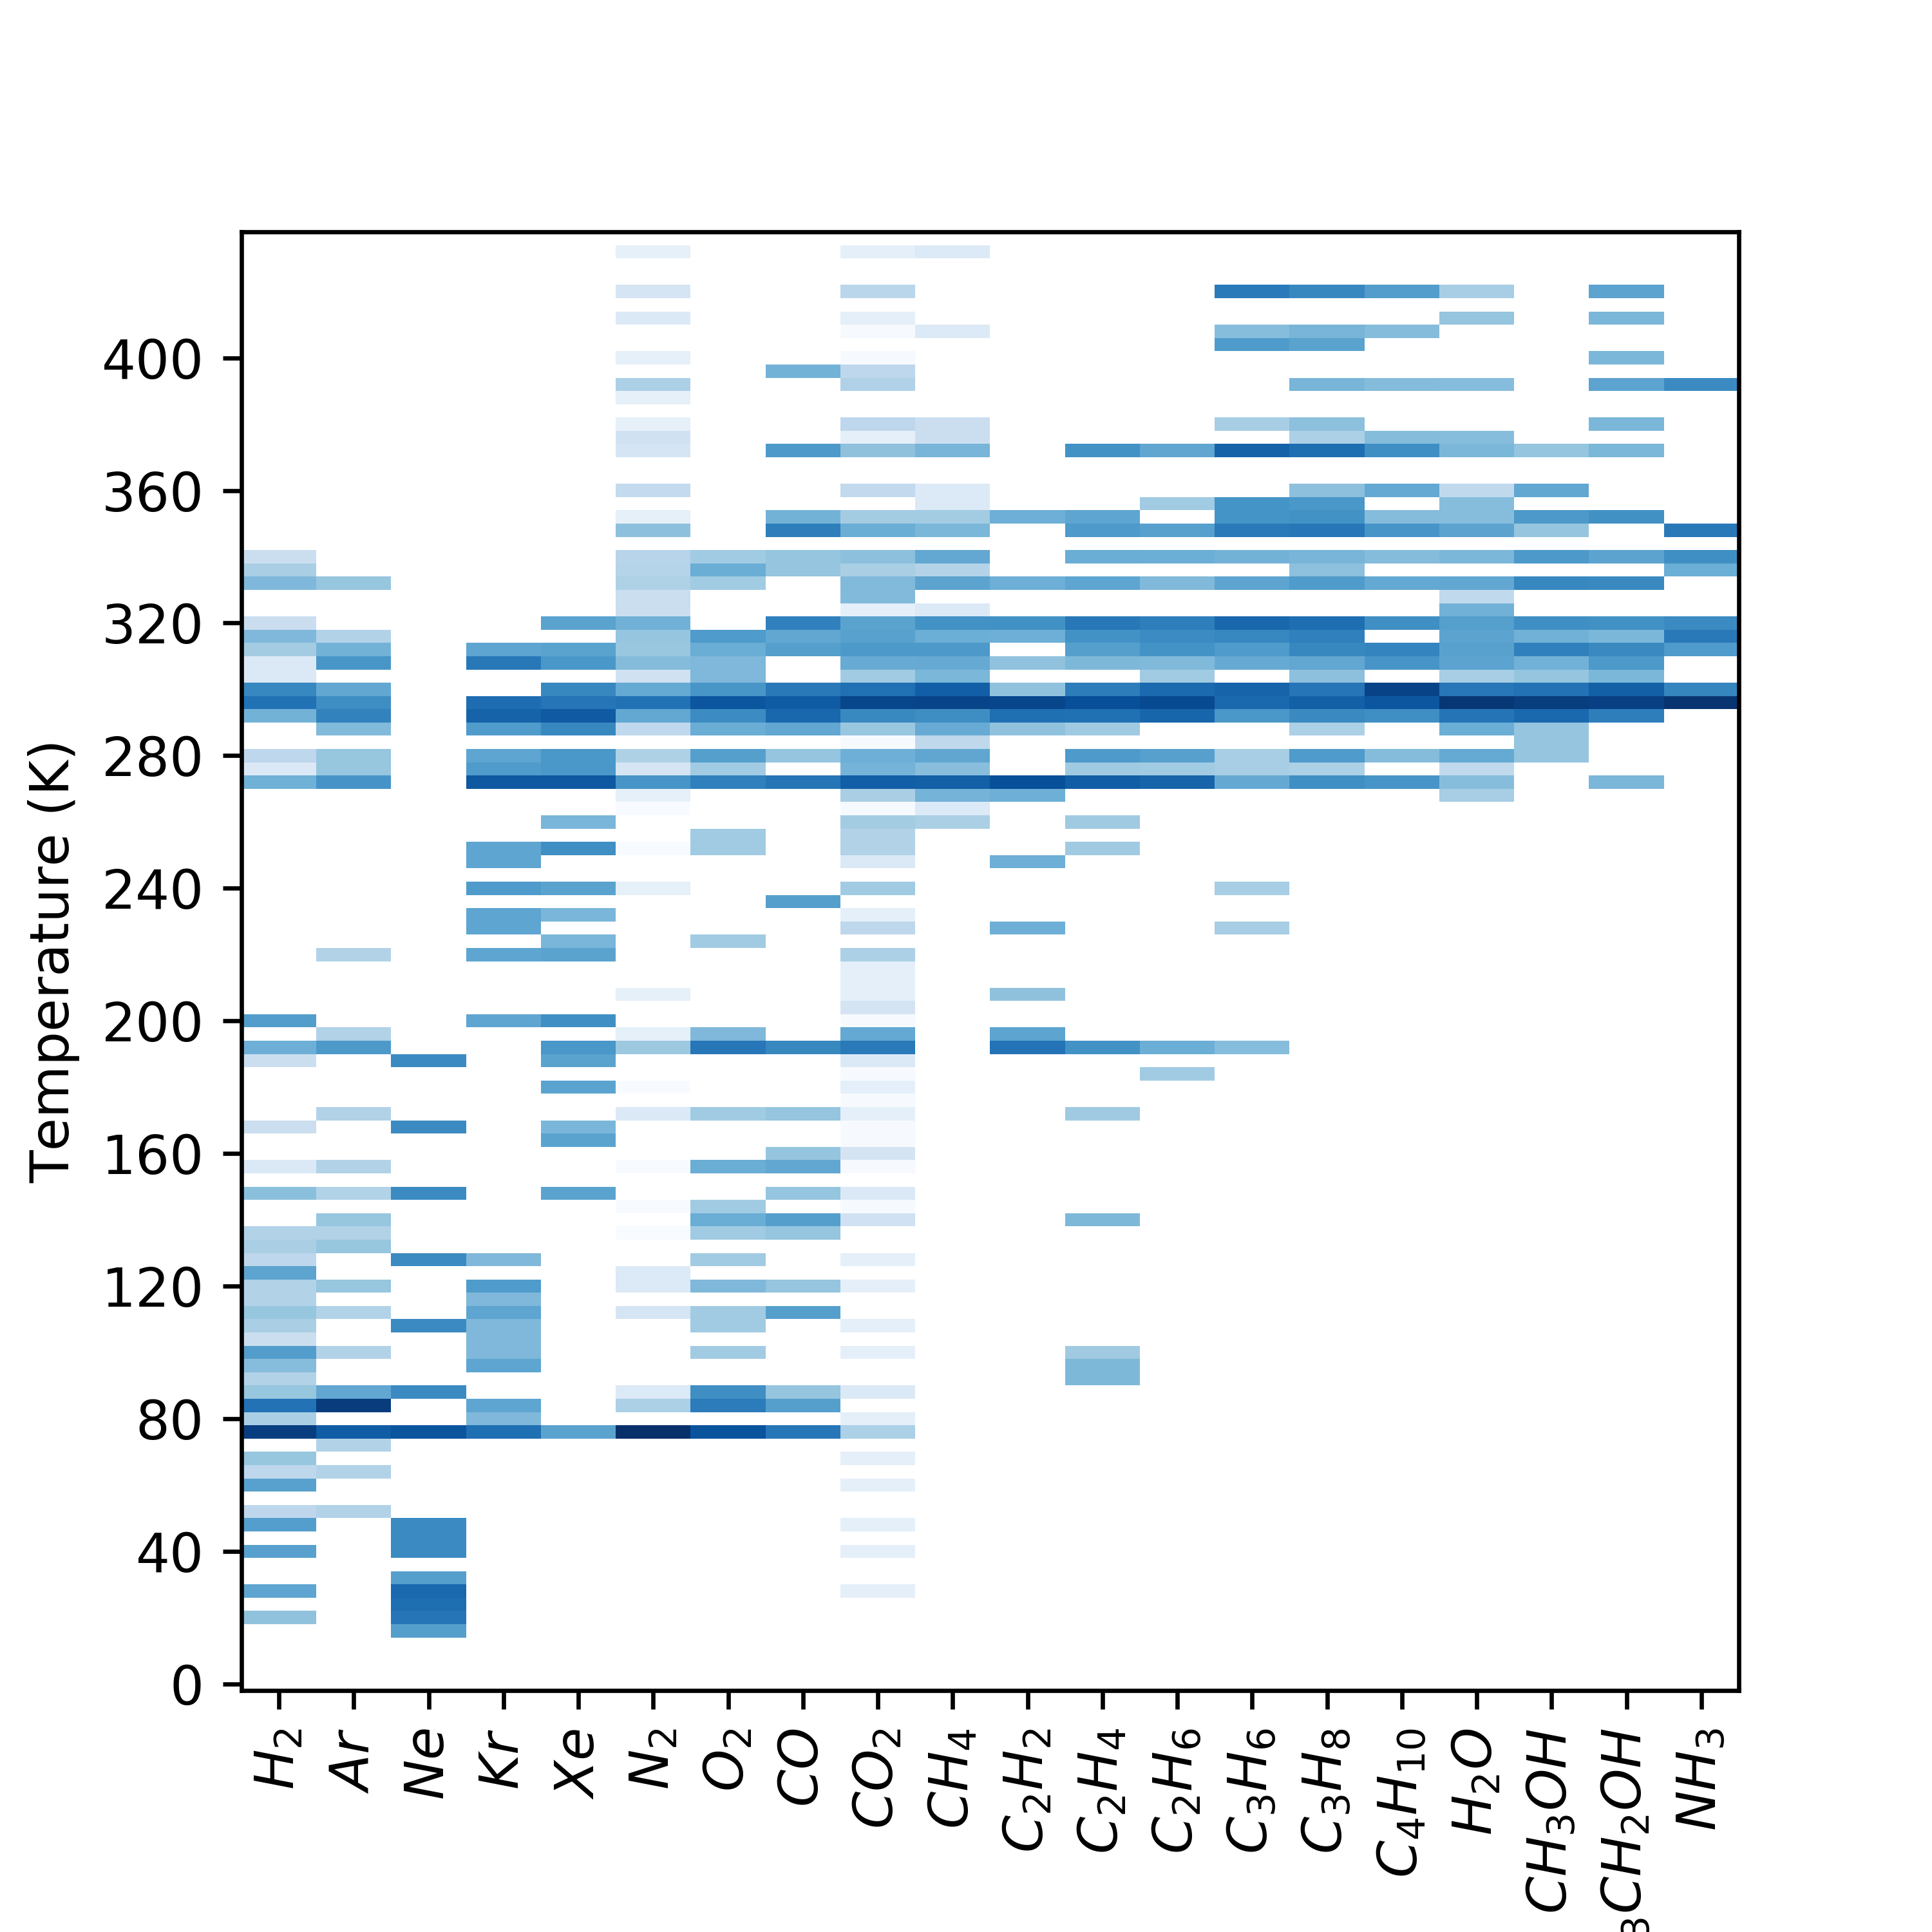
\includegraphics[width=\linewidth]{nist/nist-dataset}%
		\caption{}%
		\label{pyg:fgr:nist-dataset}
	\end{subfigure}%
	\begin{subfigure}[b]{0.45\linewidth}
		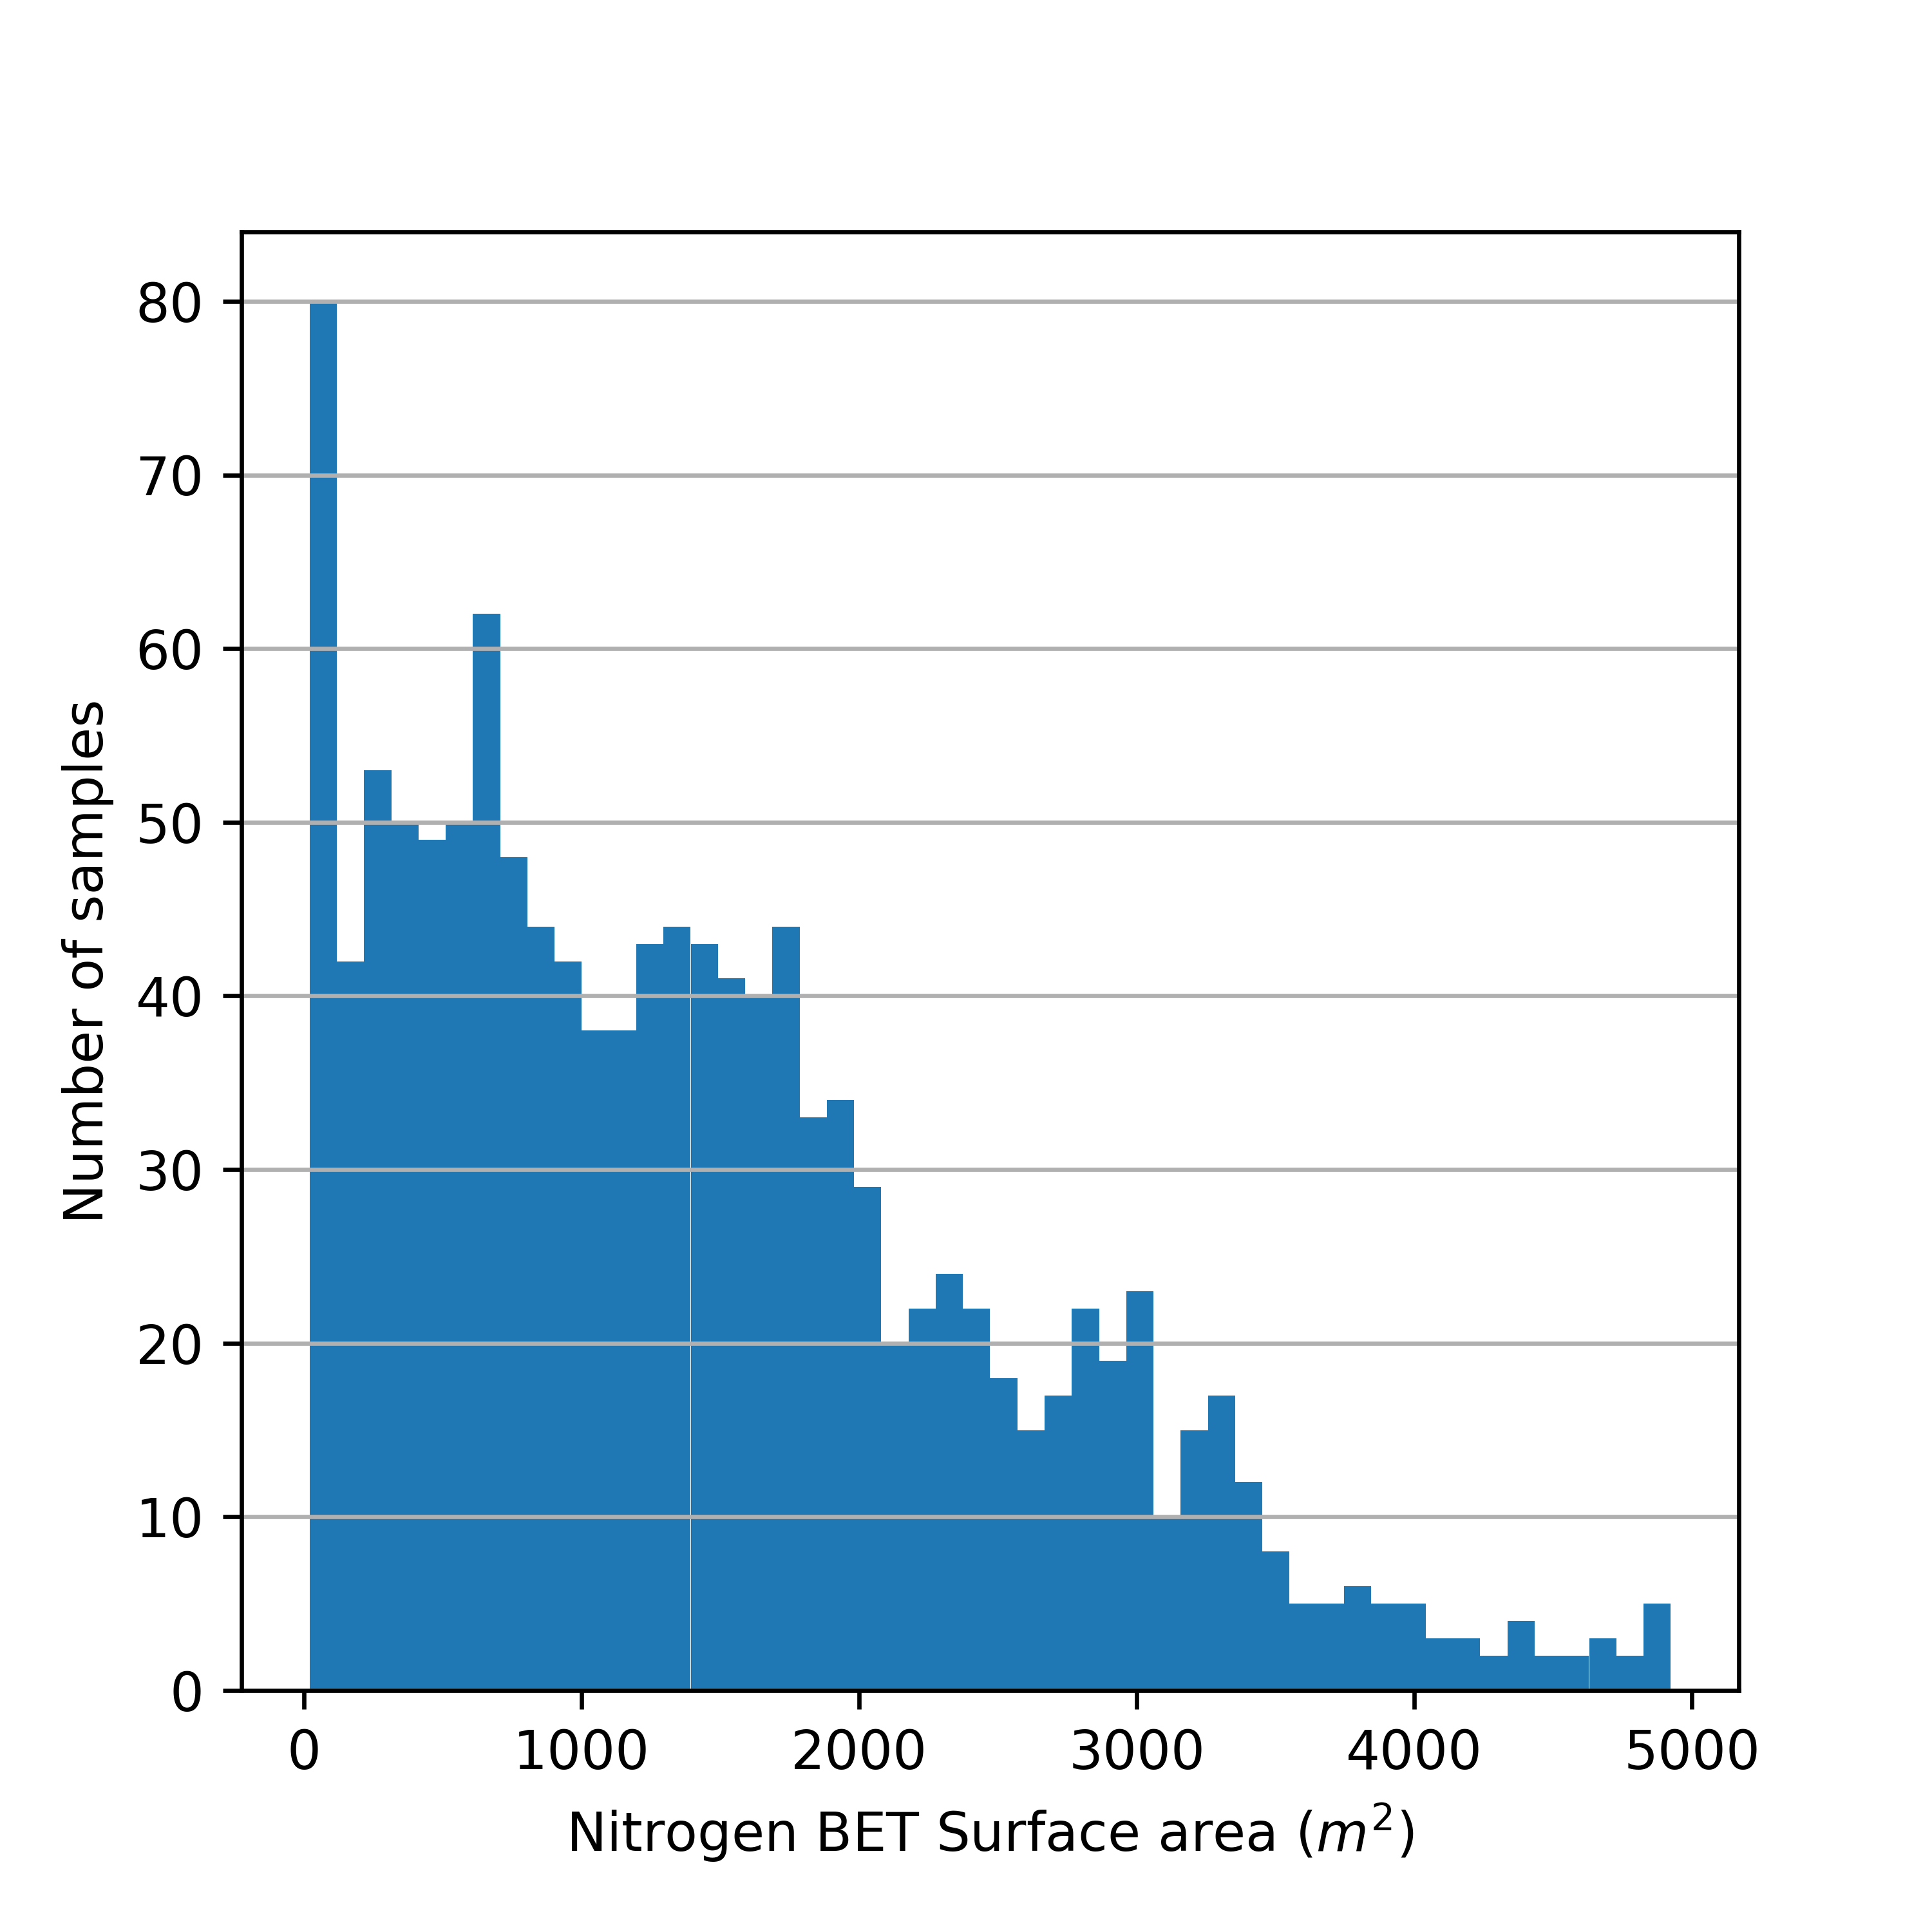
\includegraphics[width=\linewidth]{nist/nist-bet-area}%
		\caption{}%
		\label{pyg:fgr:nist-dataset-area}
	\end{subfigure}%

	\caption{A graphical description of the NIST ISODB dataset.
		(a) The selected 15800 isotherms presented per adsorbate used
		and temperature at which the measurement took place.
		(b) Calculated BET surface area with nitrogen at \SI{77}{\kelvin}
		for all available isotherms. }%
	\label{pyg:fgr:nist-set}
\end{figure}

For an initial round of data processing with pyGAPS,
only isotherms recorded with nitrogen at \SI{77}{\kelvin}
were selected. These make up \(\approx \! 3500\) datapoints,
recorded on more than 2200 materials. The BET surface area
was then computed for each isotherm, with a distribution
as seen in \autoref{pyg:fgr:nist-dataset-area}.
Unfortunately, as many isotherms do not have enough points
in the low pressure region, computing a well-defined
BET surface area is impossible. In total, only around a
third of the isotherms had enough data for this purpose.
Several materials are seen to be essentially non-porous
with around 80 isotherms recorded having a BET area of less
than \SI{100}{\metre^2\per\gram}. As expected, a decrease in
number of samples is seen with increasing surface area
reflecting the lower preponderence of highly porous
materials due to the challenges involved in their
creation. Overall, while this initial calculation does
not impart any further insights, it serves as an useful overview
of the ISODB dataset.

\subsection{A comparison between surface area calculation methods}

The Langmuir surface area is an often-reported alternative
to the, now standard, BET method area.
With such a large dataset at our disposal, we can take
the opportunity to observe the differences between results
obtained with the two methods.
If the Langmuir area is calculated with implicit parameters,
by taking the entire available isotherm for the fitting
routine, the correlation between the two methods looks
like \autoref{pyg:fgr:nist-bet-langmuir}. The two results
do not agree well, with the Langmuir surface
area usually higher than the BET value for the
same isotherm. This is a consequence of the Langmuir model
assuming adsorption up to a single monolayer with other
characteristic phenomena such as multilayer adsorption,
pore condensation or multiple types of adsorption types
unable to be accounted for. It is for this reason that the 
Langmuir \textit{should not be used} in adsorption regimes 
such as nitrogen at \SI{77}{\kelvin}.

If the partial pressure range is narrowed, by only using
points up to 0.15 \(p/p_0\), the correlation improves
dramatically, with near-overlap when the area is below
\SI{2000}{\metre^2\per\gram}. In this case the selection corresponds
to a region below the ``knee'' of an ideal BET isotherm,
before the statistical monolayer is filled.

\begin{figure}[htb]
	\centering

	\begin{subfigure}{0.42\linewidth}
		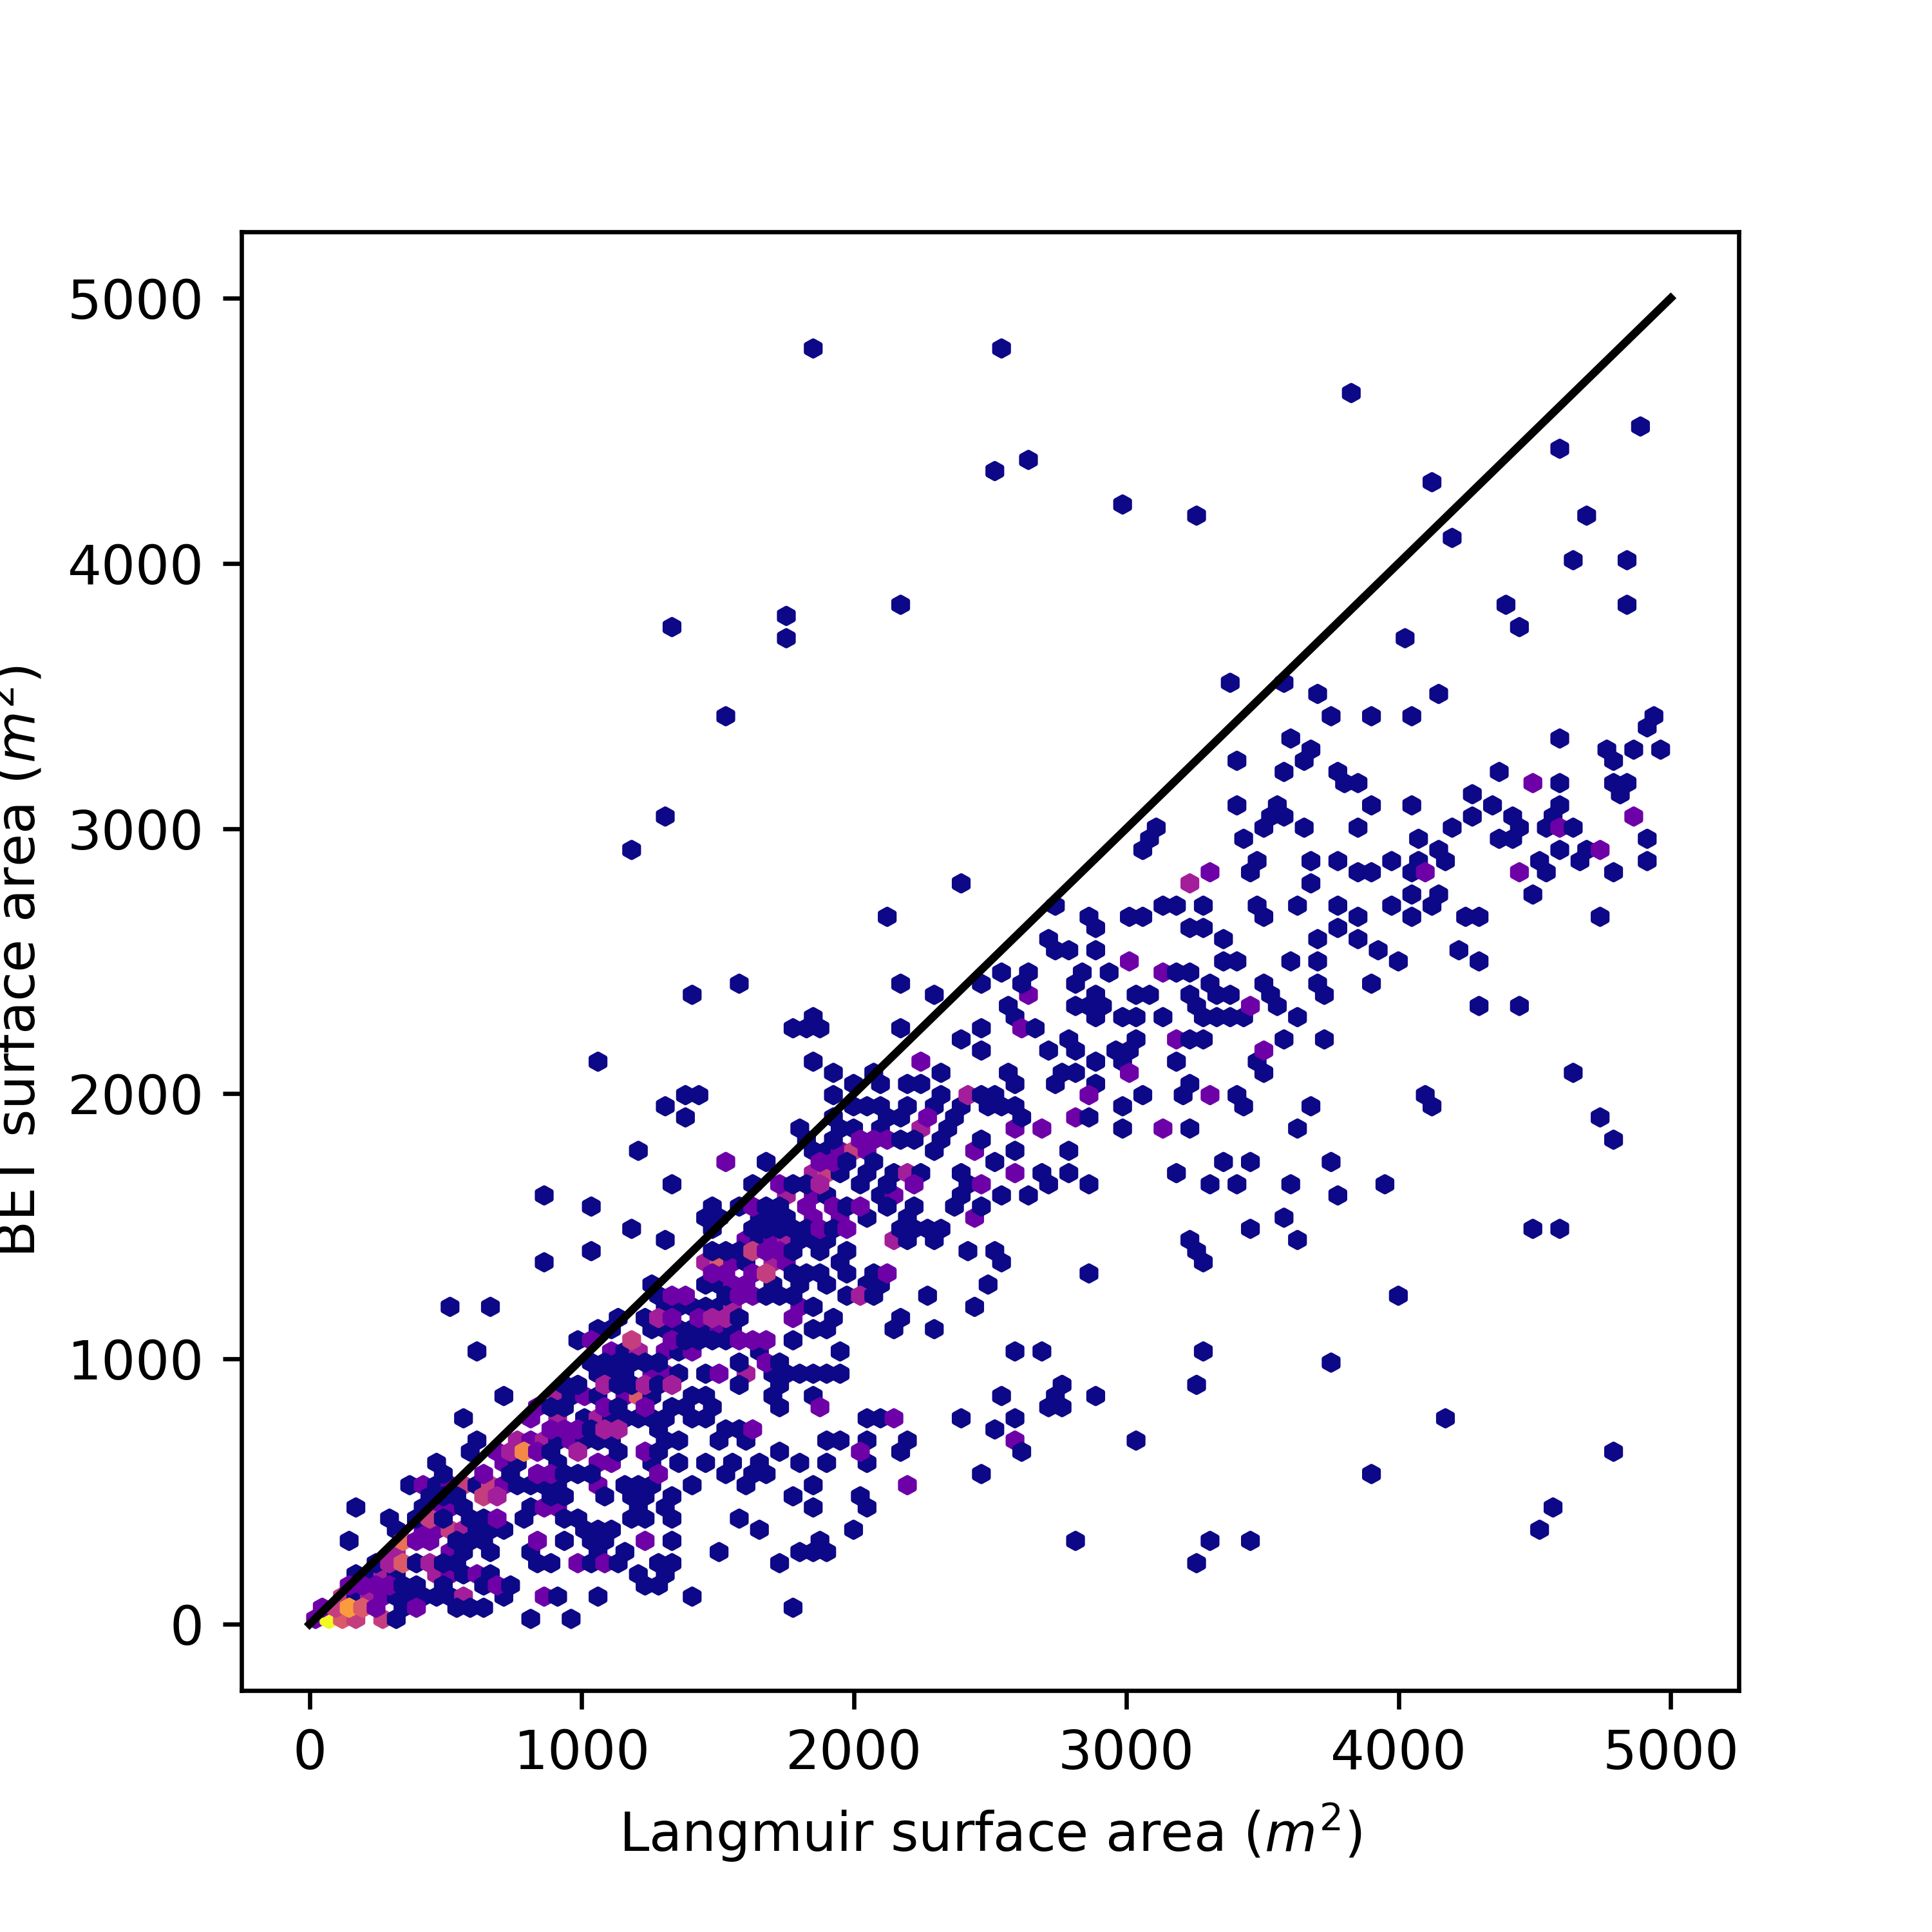
\includegraphics[width=\linewidth]{nist/nist-bet-langmuir}
		\caption{Full range}%
		\label{pyg:fgr:nist-bet-langmuir}
	\end{subfigure}%
	\begin{subfigure}{0.5\linewidth}
		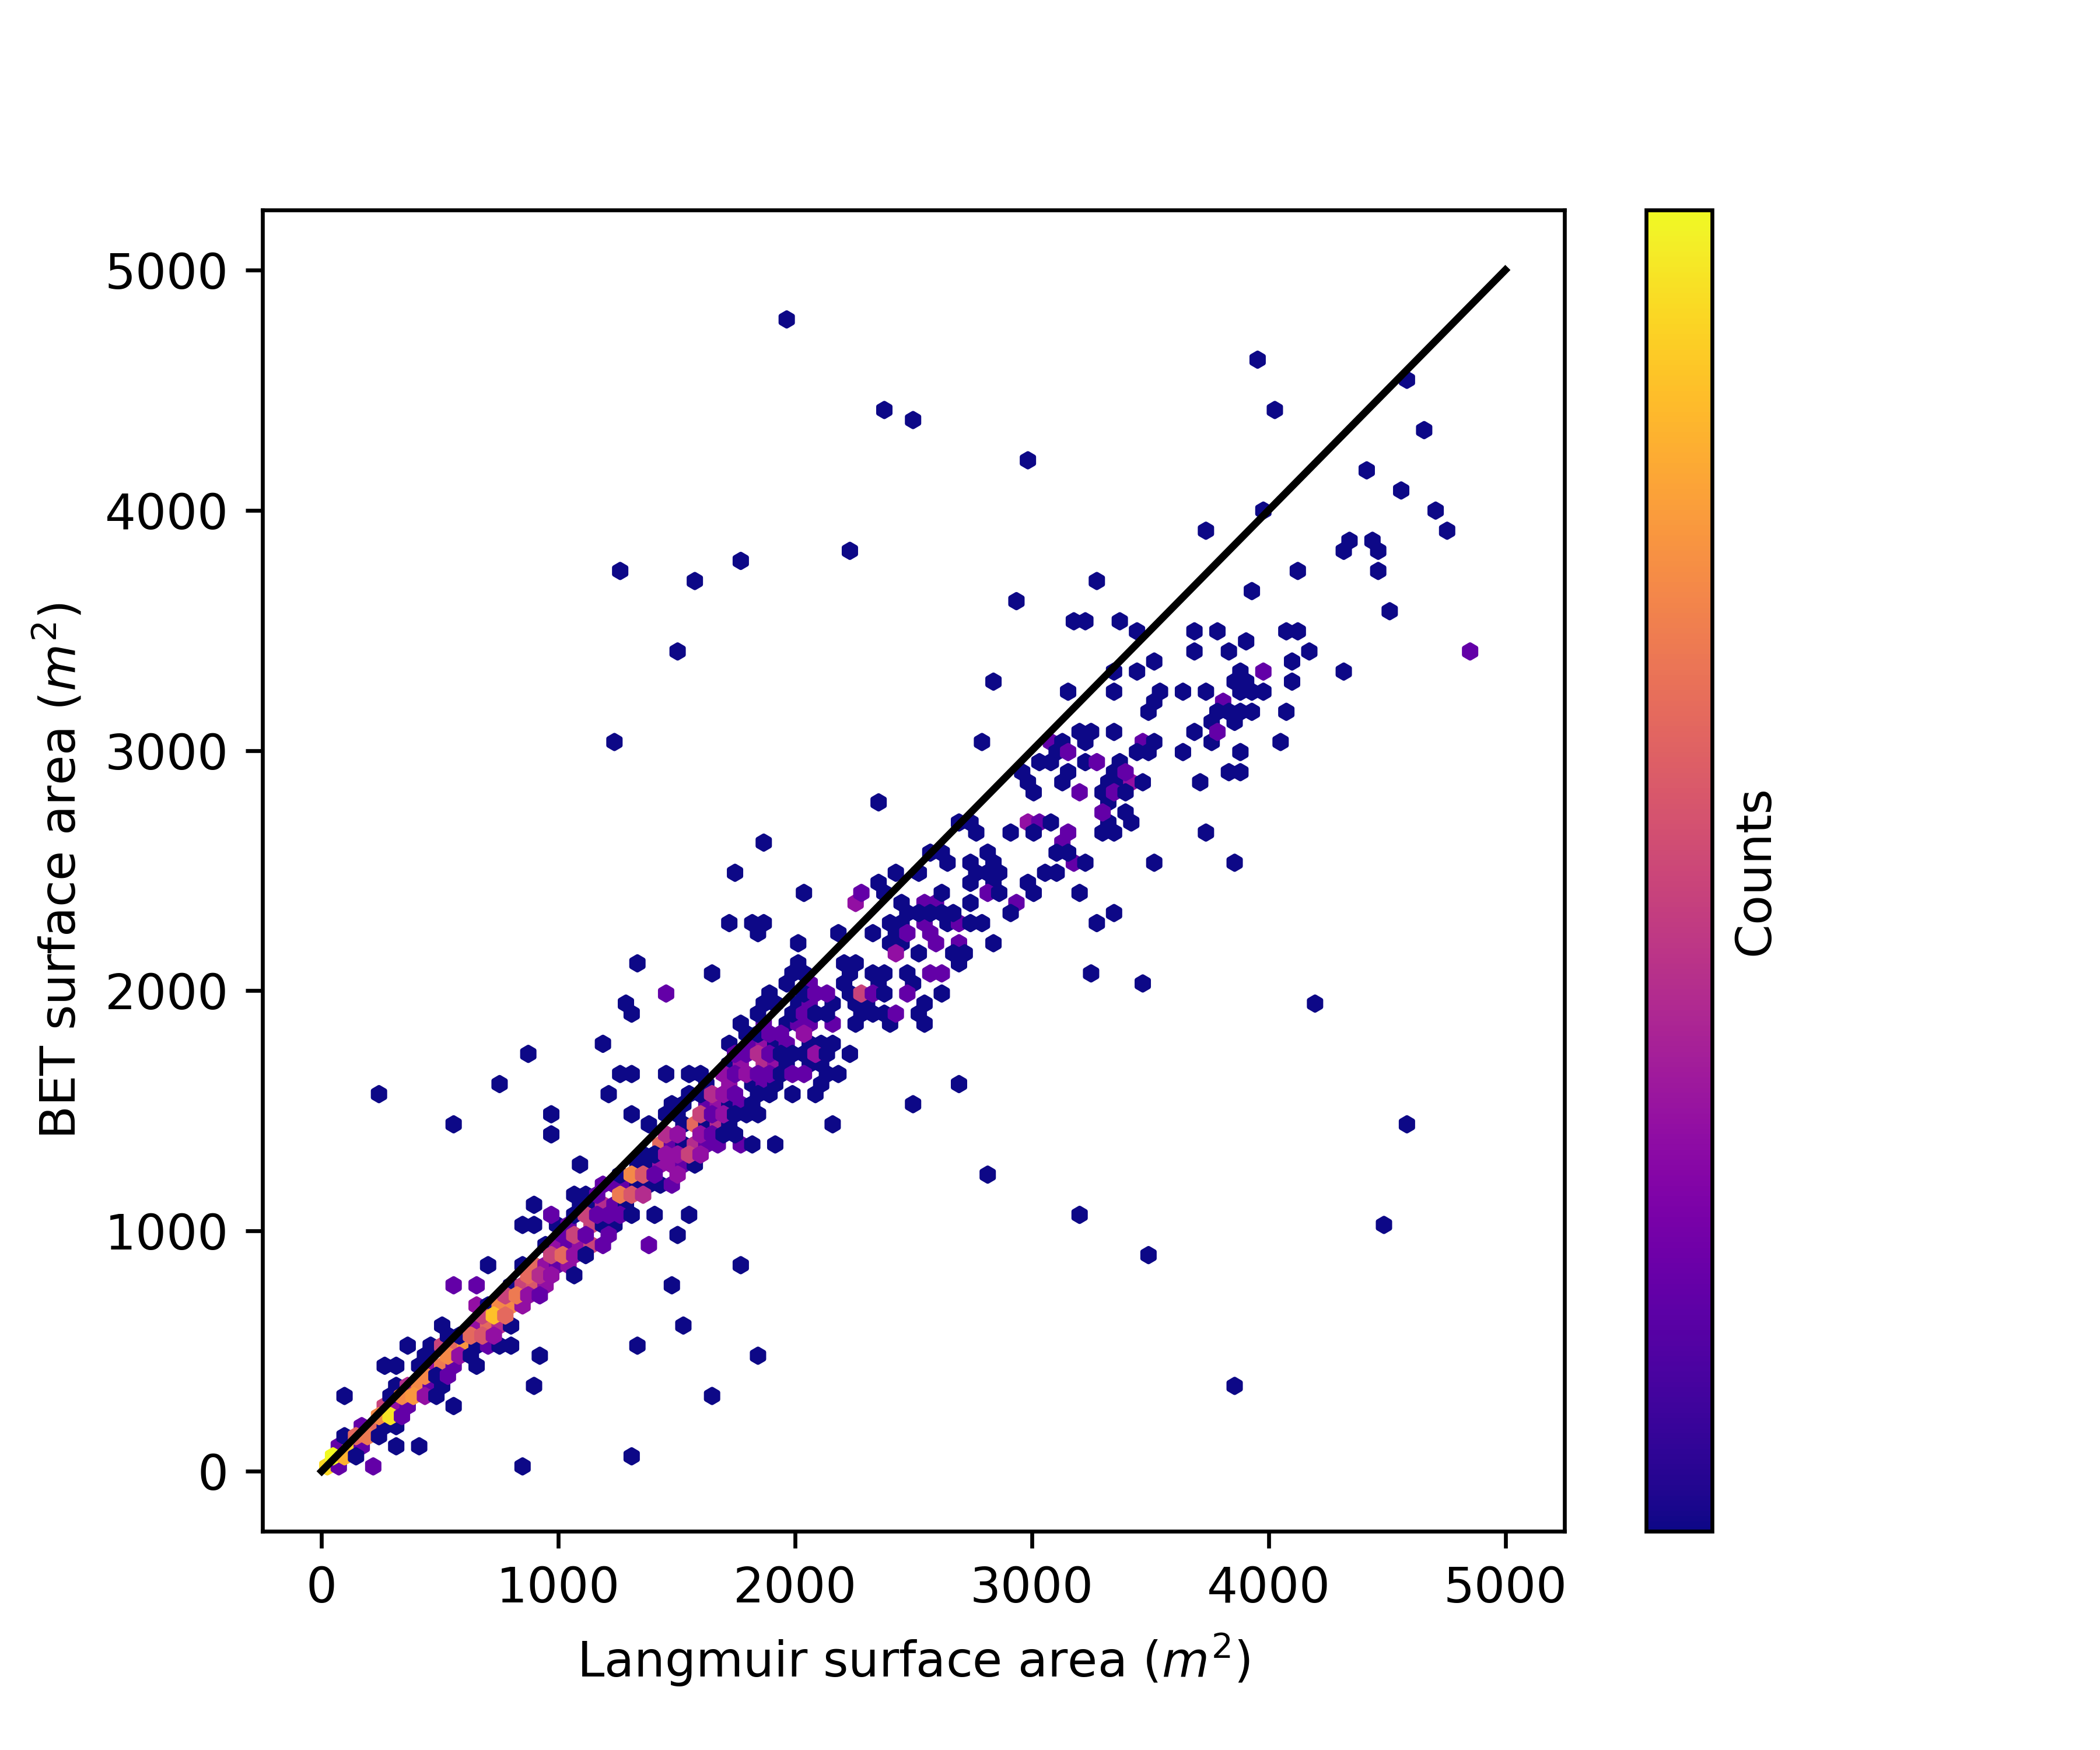
\includegraphics[width=\linewidth]{nist/nist-bet-langmuir-2}
		\caption{0--0.15 \(p/p_0\) range}%
		\label{pyg:fgr:nist-bet-langmuir-adj}
	\end{subfigure}%

	\caption{Correlation between Langmuir-calculated and
		BET-calculated surface areas. The black line is a guide
		for the eye at \(S_{Lang} = S_{BET}\).}%
	\label{pyg:fgr:nist-area-cmp}
\end{figure}

In truth, the choice of neither model is strictly
applicable to determine the accessible area of microporous
materials, due to adsorption in such samples being dominated
by pore filling mechanisms rather than monolayer formation.
However, as detailed by
\citet{rouquerolBetEquationApplicable2007}
and then also shown through comparing simulated and
experimental data by
\citet{waltonApplicabilityBETMethod2007}, the results
produced by judicious application of such models can relate
well to the actual surface areas of MOFs.

\subsection{Variability of the dataset}

Before a deeper dive into attempting to relate adsorption isotherm
derived parameters to structural properties, an analysis of the
reliability of the data from the NIST ISODB should be performed.

\begin{wrapfigure}{h}{0.5\textwidth}
	\centering
	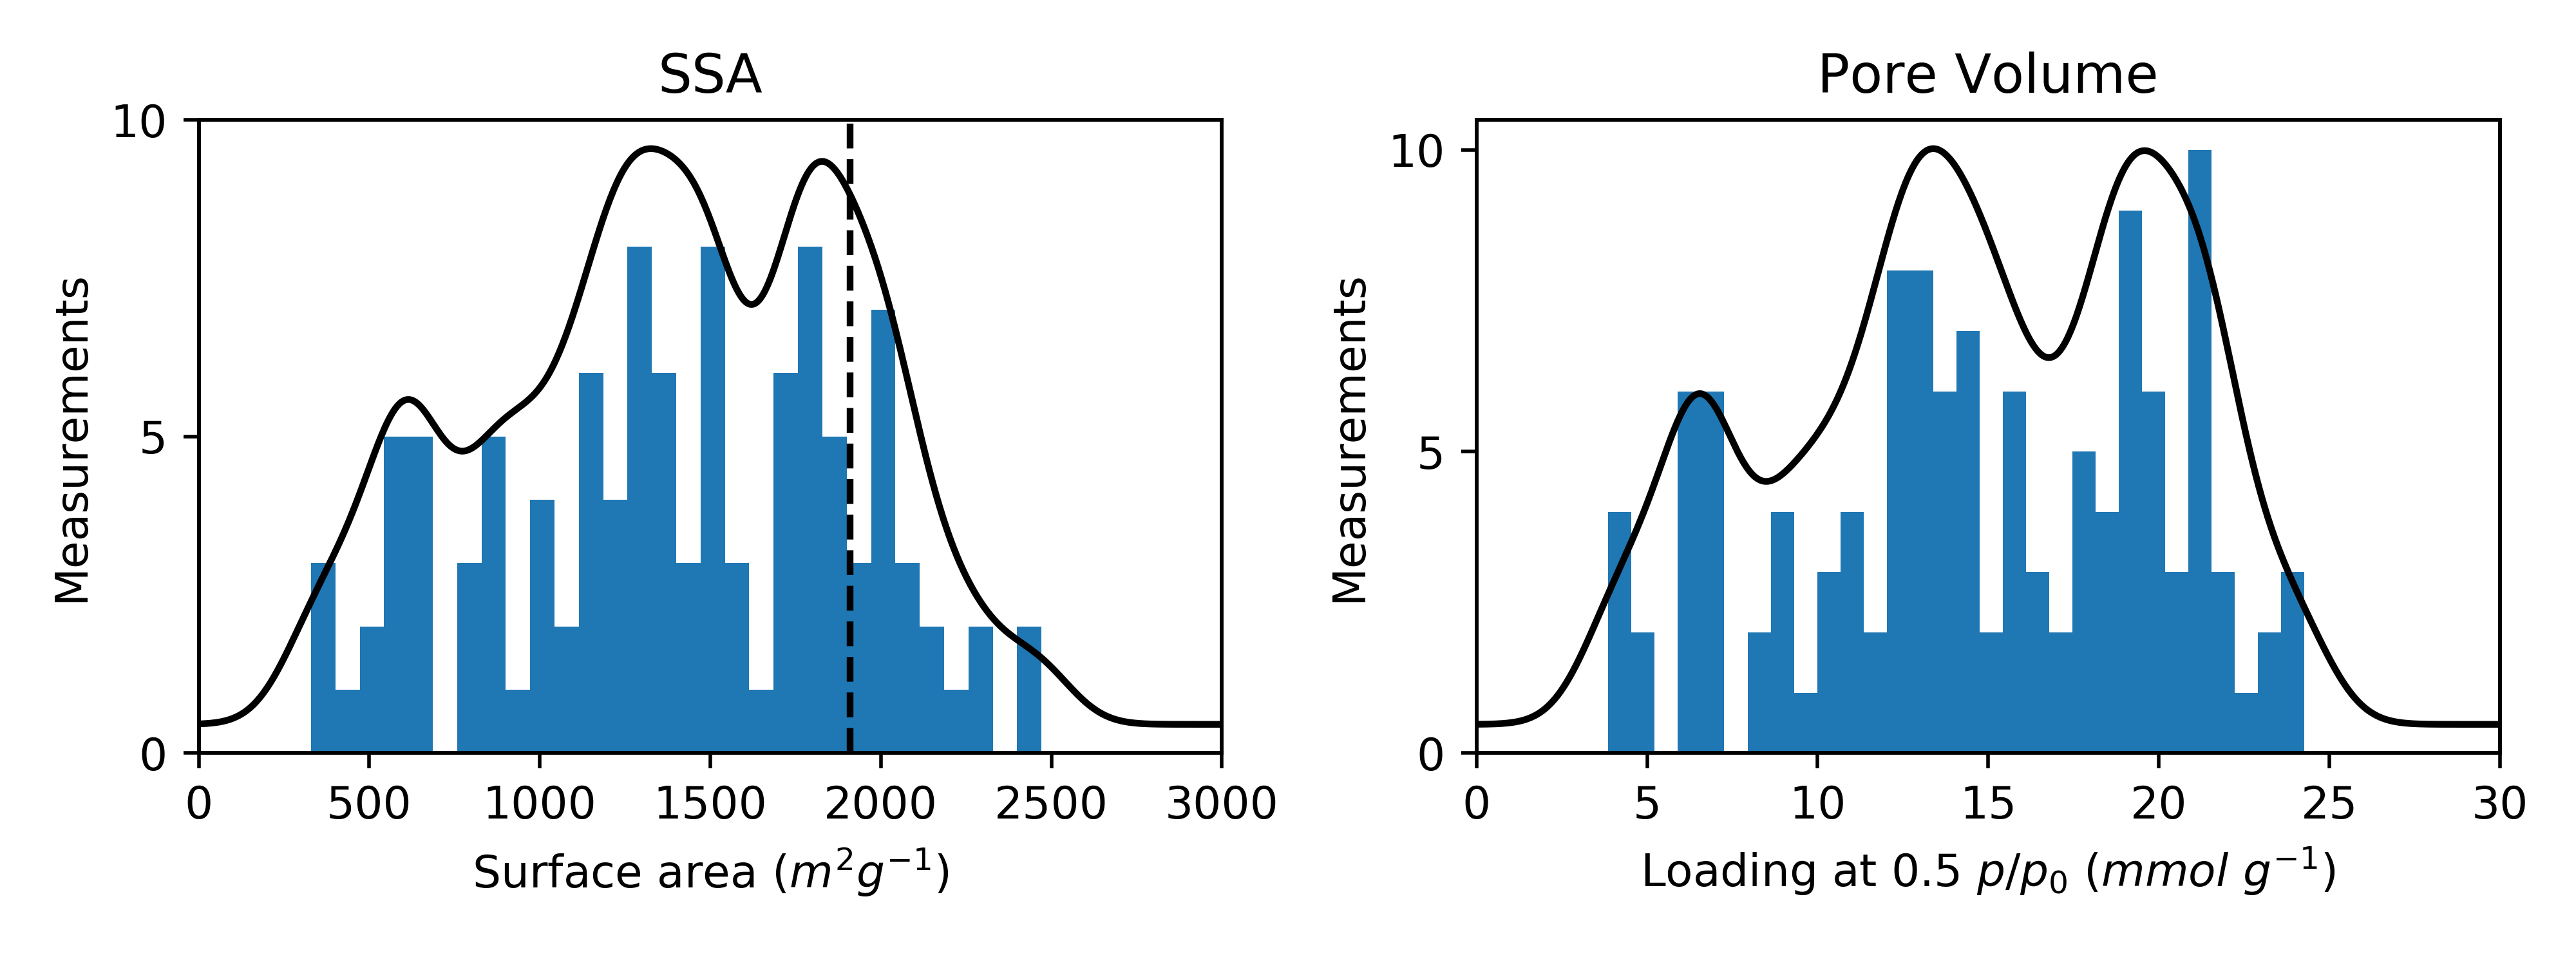
\includegraphics[width=0.47\textwidth]{nist/nist-area-cubtc}%
	\caption{A histogram and estimate of the probability density
		function for (top) BET surface area and (bottom) loading
		at half saturation pressure for CuBTC. The black dotted line
		is the simulated surface area of this MOF.}%
	\label{pyg:fgr:nist-area-cubtc}
\end{wrapfigure}

The material with the most recorded isotherms is CuBTC, with
122 datapoints. A spread of the calculated BET surface areas,
together with the ``ideal'' area of this MOF as obtained
through simulations~\cite{parkHowReproducibleAre2017} is
presented in \autoref{pyg:fgr:nist-area-cubtc}.
To verify if the variability is due to uncertainty in the
surface area calculation a secondary metric, namely the
capacity at 0.5 \(p/p_0\) has been calculated and its
distribution plotted alongside that of the BET area. The
identical trends in both parameters show that there is an
inherent uncertainty in the dataset. The results not only
have a large standard deviation, but also do not have a
typical normal distribution one would expect from repeated
sampling of a physical property.

Instead, three normal distributions appear to emerge, one with a
median around \SI{500}{\metre^2\per\gram}, a second around \SI{1300}{\metre^2\per\gram}
and a third with a median around \SI{1900}{\metre^2\per\gram} which also
corresponds to the nitrogen accessible surface area determined through
simulation. As the NIST data also records the DOI for each isotherm, each
measurement can be traced to the publication it originated in.
By cherry-picking several studies from each normal distribution
we can find that the low surface areas correspond to data
measured on modified versions of CuBTC, such as shaped
samples (\SI{640}{\metre^2\per\gram})~\cite{liSeparationCO2CH42014}, hollow
nanoparticles (\SI{450}{\metre^2\per\gram})~\cite{liControllableSynthesisMetal2013}
or nanoplates
(\SI{803}{\metre^2\per\gram})~\cite{pengSurfactantdirectedAssemblyMesoporous2012}.
Studies selected from materials with higher surface area
showed no consistent underlying cause for the variability,
although some can be accounted for through synthesis method
such as mechanosynthesis
(\SI{1700}{\metre^2\per\gram})~\cite{klimakowMechanochemicalSynthesisMetal2010},
or structural defects (\SI{2050}{\metre^2\per\gram})~\cite{barinDefectCreationLinker2014}.

To extend the analysis to other materials, MOFs with
at least 8 recorded nitrogen isotherms were selected, resulting in
16 materials. A violin plot with the results of the calculation for
these datapoints is presented in \autoref{pyg:fgr:nist-area-repr}.
The blue points mark the surface area of the material as
obtained from literature of simulated values or, if not available,
the original synthesis paper of the MOF in question.
It is obvious that, in most cases, there is a large spread in
the calculated values, with some samples such as IRMOF-1,
IRMOF-3 and MIL-101(Cr) having a surface area anywhere
between \SIrange{200}{5000}{\metre^2\per\gram}. Other materials,
such as ZIF-8, the MIL-53 family
and MIL-100(Fe) have less variability in their surface areas,
although can still be shifted by 200 to \SI{500}{\metre^2\per\gram}.

\begin{figure}[tb]
	\centering
	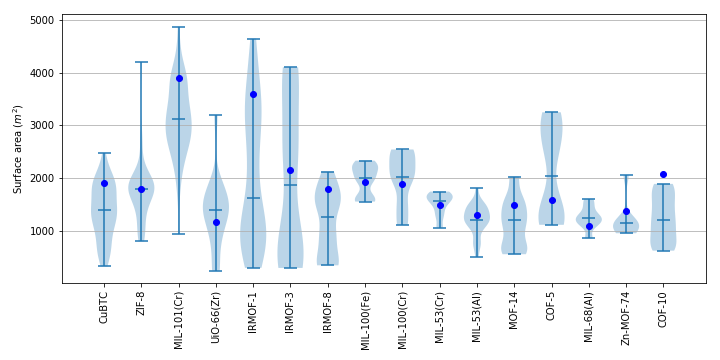
\includegraphics[width=\linewidth]{nist/nist-area-repr}%
	\caption{A violin plot of the calculated surface areas for
		all available nitrogen isotherms on the top 16 MOFs.
		The top and bottom lines in each plot are the limits for
		the surface area values. The shaded area is a kernel-density estimate
		of the probability density function using Gaussian kernels.
		The median of each dataset is displayed as the horizontal line
		between the two limits. Finally, the round blue point is the
		BET surface area of the material as reported in literature through
		simulation or optimised synthesis.}%
	\label{pyg:fgr:nist-area-repr}
\end{figure}

Similar concerns have been
raised for \ce{H2}~\cite{broomIrreproducibilityHydrogenStorage2016}
and \ce{CO2}~\cite{espinalMeasurementStandardsData2013} measurements.
Recently, Sholl and co-workers~\cite{parkHowReproducibleAre2017}
have published a report putting into question the reproducibility
or adsorption isotherms, using \ce{CO2} adsorption data from the
NIST adsorption database. Their findings highlight a large
variability inherent
to reported isotherms as on average \textit{``one in five \ce{CO2}
	isotherms [\ldots] cannot be used to provide information that
	is qualitatively reliable about the properties of the material''}.
However, in their paper they do not explore the reasons behind the
origin of such large variations.

The underlying cause for the poor reproducibility of adsorption
isotherms, particularly those measured on metal organic frameworks,
is not easy to pinpoint. A large contribution to this divergence
is likely accounted for through the variation introduced by the
sample preparation method and adsorption apparatus.
For example, a recent NIST interlaboratory study in which \ce{CO2}
isotherms were recorded on a reference
material~\cite{nguyenReferenceHighpressureCO22018}, received six
out of thirteen initial datasets outside the uncertainty range.
Errors were determined to arise from sample mass measurement,
insufficient activation conditions or improper choice of an
equation of state. Other method-specific sources of error exist,
such as the lack of a buoyancy correction when using a
gravimetric system or a void volume correction when using
a volumetric system, both of which can made if an accurate
determination of sample skeletal density is performed. Finally,
small differences in thermal gradients, pressure transducer
readings, and even the altitude at which the measurement takes place
(if a phase change bath is used to control temperature)
can also impact the final isotherm.

Such variation is likely minimised when using state-of-the-art
adsorption equipment, which eliminates many of the concerns
associated with adsorption methodology. \textit{In situ}
activation, internal consistency checks for pressure transducers,
automatic measurement of skeletal density and associated
corrections, reference cells for saturation pressure determination
and many other sanity checks are implemented in these machines.

However, it is often the case that the most important factor
in the repeatability of MOF adsorption isotherms
is not the measurement procedure, but rather the material itself.
As evidenced by the closer look at the CuBTC dataset, synthesis
method, crystalinity, material form, particle size and contribution
of defects all have an impact on the resulting adsorption behaviour
of the material. Furthermore, IRMOF-3, the sample with the 
highest variability in the dataset is known to possess structural
flexibility, with the activation procedure responsible for 
any number of states from a completely open to a completely closed
framework~\cite{nelsonSupercriticalProcessingRoute2009}. In this 
sense, such an analysis of a large MOF dataset can point out 
which materials tend to be resistant (or susceptible) to the 
aforementioned sources of variability 
and can lend themselves to use as standard or reference materials.